\documentclass[a4paper,12pt]{book}


%************
%* packages *
%************


\usepackage[latin1]{inputenc}
\usepackage[italian]{babel}
\usepackage{fancyhdr}
\usepackage{verbatim}
\usepackage{float}
\usepackage{subfigure}
\usepackage[stable]{footmisc}
\usepackage[hang,small,sf]{caption}
\usepackage{cite}
\usepackage{acronym}
\usepackage{sectsty}
\usepackage{listings}
\usepackage[usenames]{color}
\usepackage{graphicx}
\usepackage[italian]{varioref}
\usepackage{lmodern}
\usepackage[left=2.5cm,right=2.5cm,bottom=2.8cm]{geometry}
\usepackage{colortbl}
\usepackage{booktabs,graphicx,pgfgantt,tikz-uml}
\usepackage{fontspec}
\usetikzlibrary{shapes,arrows,chains}
\usepackage{acronym}


%*****************
%* nuovi comandi *
%*****************

\newcommand{\abs}[1]{\left|#1\right|}                               % modulo
\newcommand{\dato}{\left|\right.}                                   % probabilit\`{a} condizionata
\newcommand{\fun}[1]{\mathrm{#1}}                                   % stile funzione
\newcommand{\imp}{\;\;\Longrightarrow\;\;}                          % implicazione
\newcommand{\norma}[1]{\left\| #1 \right\|}                         % norma
\newcommand{\prob}[1]{\mathrm{P}\!\left[#1\right]}                  % probabilit\`{a}
\newcommand{\expect}[1]{\mathrm{E}\!\left[#1\right]}                % aspettazione
\newcommand{\sse}{\;\;\Longleftrightarrow\;\;}                      % se e solo se
\newcommand{\vect}[1]{{\boldsymbol{\mathrm{#1}}}}                   % stile vettore
\newcommand{\real}[1]{\fun{Re}\left[#1\right]}                      % parte reale
\newcommand{\imag}[1]{\fun{Im}\left[#1\right]}                      % parte immaginaria
\newcommand{\Dim}[1]{\fun{dim}\left[#1\right]}                      % dimensione di una matrice
\newcommand{\Det}[1]{\fun{det}\left[#1\right]}                      % determinante di una matrice
\newcommand{\Ker}[1]{\fun{ker}\left[#1\right]}                      % ker di una matrice
\newcommand{\rango}[1]{\fun{rango}\left[#1\right]}                  % rango di una matrice
\newcommand{\scalare}[2]{\left\langle #1, #2 \right\rangle}         % prodotto scalare
\newcommand{\blbrace}{\left  \lbrace}                               % parentesi graffa sinistra grande
\newcommand{\brbrace}{\right \rbrace}                               % parentesi graffa destra grande
\newcommand{\sinc}{\fun{sinc}}                                      % sinc
\newcommand{\rect}{\fun{rect}}                                      % rect
\newcommand{\rcos}{\fun{rcos}}                                      % rcos
\newcommand{\sgn}{\fun{sgn}}                                        % sgn
\newcommand{\N}{\mathbb{N}}                                         % insieme dei numeri naturali
\newcommand{\Z}{\mathbb{Z}}                                         % insieme dei numeri interi
\newcommand{\Q}{\mathbb{Q}}                                         % insieme dei numeri razionali
\newcommand{\R}{\mathbb{R}}                                         % insieme dei numeri reali
\newcommand{\C}{\mathbb{C}}                                         % insieme dei numeri complessi
\newcommand{\seq}[2][n]{#2_{0}, #2_{1}, \ldots, \, #2_{#1}}         % sequenza
\newcommand{\Span}[2][n]
{\fun{span} \blbrace #2_{1}, #2_{2}, \ldots, \, #2_{#1} \brbrace}   % spazio generato
\newcommand{\ddt}{\frac{\fun{d}}{\fun{dt}}}                         % derivata
\newcommand{\Div}[2]{#1 \; \mid \; #2}                              % divide
\newcommand{\MCD}[2]{\fun{MCD}\(#1, #2\)}                           % massimo comun divisore
\newcommand{\mcm}[2]{\fun{mcm}\(#1, #2\)}                           % minimo comune multiplo
\newcommand{\goodgap}{
                      \hspace{\subfigtopskip}
                      \hspace{\subfigbottomskip}
                     }                                              % interlinea opportuna per le sottofigure
\newcommand{\eng}[1]{\emph{#1}}                                   % inglese
\newcommand{\virg}[1]{``#1"}                                        % fa una citazione tra virgolette
%\newcommand{\unit}[2]($\frac{\text{#1}}{\text{#2}}$)                % unit\`{a} di misura
\newcommand{\textttvar}[1]{{\ttvar #1}}

\definecolor{gray}{gray}{0.9}
\newcommand{\listato}[1]{\lstset{language=#1, numbers=left, numberstyle=\tiny, stepnumber=2, numbersep=5pt, numberblanklines=false, xleftmargin=5pt, captionpos=b, stringstyle=\ttfamily, columns=flexible, showstringspaces=false, tabsize=2, frame=single, framerule=0pt, backgroundcolor=\color{gray}, basicstyle=\small}}

%****************************
%* ridefinizioni di comandi *
%****************************

\renewcommand{\(}{\left(}                                     % parentesi tonda sinistra grande
\renewcommand{\)}{\right)}                                    % parentesi tonda destra grande
\renewcommand{\[}{\left[}                                     % parentesi quadra sinistra grande
\renewcommand{\]}{\right]}                                    % parentesi quadra destra grande
\renewcommand{\exp}[1]{\fun{e}^{#1}}                          % esponenziale
\renewcommand{\gcd}[2]{\fun{gcd}\(#1, #2\)}                   % massimo comun divisore

\renewcommand{\lstlistingname}{Codice}
\renewcommand{\lstlistlistingname}{Elenco dei listati codice}

\newfont{\ttvar}{cmvtt10 scaled 1200}     % nuovo carattere tipi courier a spaziatura variabile per le dimostrazioni


% interlinea
%\renewcommand{\baselinestretch}{1.25}

% margini
%\setlength{\topmargin}{-1cm}
%\setlength{\textheight}{24cm}
%\setlength{\textwidth}{17cm}
%\setlength{\oddsidemargin}{-0.6cm}
%\setlength{\evensidemargin}{-0.6cm}
%\setlength{\headsep}{1.0cm}
%\setlength{\footskip}{1.0cm}
%\setlength{\parindent}{0.7cm}
%\setlength{\captionmargin}{0.7cm}

% margini senato
\textwidth       =  14.50 cm            % larghezza 21 cm - 4 cm (sinistro) - 2.5 (destro)
\textheight      =  23.10 cm            % altezza 29.7 cm - 3 cm (superiore) - 2 (inferiore)
\topmargin       =   0.00 cm            % margine superiore 3 cm diminuito di 1 inch
\oddsidemargin   =   1.46 cm            % margine sinistro 4 cm diminuito di 1 inch
\evensidemargin  =  -0.04 cm            % margine destro 2.5 cm diminuito di un inch
%\renewcommand{\baselinestretch}{1.25}   % interlinea
\setlength{\headsep}{1.0cm}
\setlength{\footskip}{1.0cm}
\parindent = 0.7cm
\captionmargin = 0.7cm



% stile pagina
\pagestyle{fancy}
\renewcommand{\chaptermark}[1]{\markboth{\chaptername\ \thechapter.\ #1 }{}}
\renewcommand{\sectionmark}[1]{\markright{\thesection\ #1}{}}
\fancyhead{}
\fancyhead[LE,RO]{\sffamily \thepage}
\fancyhead[RE]{\sffamily \leftmark}
\fancyhead[LO]{\sffamily \rightmark}
\fancyfoot{}

% ridefinisco lo stile plain
\fancypagestyle{plain}{ \fancyhead{} \fancyfoot{}
\fancyfoot[C]{\sffamily \thepage}
\renewcommand{\headrulewidth}{0pt}}

% stile per i titoli
\allsectionsfont{\sffamily \raggedright}

% definisco i colori
\definecolor{light_yellow}{rgb}{1,1,0.7}
\definecolor{dark_yellow}{rgb}{1,1,0.5}
\definecolor{my_green}{rgb}{0,0.6,0}
\definecolor{my_red}{rgb}{0.8,0,0}

% definisco il codice sql
\lstset{basicstyle=\small\ttfamily,language=SQL, keywordstyle=\color{blue},commentstyle=\color{blue}, stringstyle=\color{my_green}}

\usepackage{xcolor}

\colorlet{punct}{red!60!black}
\definecolor{background}{HTML}{FFFCEE}
\definecolor{table}{HTML}{CCCCCC}
\definecolor{delim}{RGB}{20,105,176}
\colorlet{numb}{green!60!black}

\lstdefinelanguage{json}{
    basicstyle=\normalfont\ttfamily,
    numbers=left,
    numberstyle=\scriptsize,
    stepnumber=1,
    numbersep=8pt,
    showstringspaces=false,
    breaklines=true,
    frame=lines,
    backgroundcolor=\color{background},
    stringstyle=\color{red}\ttfamily,
    morestring=[b]',
    morestring=[b]",
    literate=
     *{0}{{{\color{numb}0}}}{1}
      {1}{{{\color{numb}1}}}{1}
      {2}{{{\color{numb}2}}}{1}
      {3}{{{\color{numb}3}}}{1}
      {4}{{{\color{numb}4}}}{1}
      {5}{{{\color{numb}5}}}{1}
      {6}{{{\color{numb}6}}}{1}
      {7}{{{\color{numb}7}}}{1}
      {8}{{{\color{numb}8}}}{1}
      {9}{{{\color{numb}9}}}{1}
      {:}{{{\color{punct}{:}}}}{1}
      {,}{{{\color{punct}{,}}}}{1}
      {\{}{{{\color{delim}{\{}}}}{1}
      {\}}{{{\color{delim}{\}}}}}{1}
      {[}{{{\color{delim}{[}}}}{1}
      {]}{{{\color{delim}{]}}}}{1}
}
\lstset{numbers=left, numberstyle=\scriptsize, stepnumber=1, numbersep=5pt,
    xleftmargin=3.0ex}
\lstdefinelanguage{JavaScript}{
  backgroundcolor=\color{background},
  frame=lines,
  basicstyle=\ttfamily\footnotesize,
  keywords={typeof, new, true, false, catch, function, return, null, catch,%
  switch, default, var, if, in, while, do, else, case, break},
  keywordstyle=\color{blue}\bfseries, ndkeywords={class, export, boolean, throw, implements, import, this},
  ndkeywordstyle=\color{darkgray}\bfseries,
  identifierstyle=\color{black},
  sensitive=false,
  comment=[l]{//},
  morecomment=[s]{/*}{*/},
  commentstyle=\color{purple}\ttfamily,
  stringstyle=\color{red}\ttfamily,
  morestring=[b]',
  morestring=[b]"
} 





\begin{document}

\begin{titlepage}
\begin{center}
% Upper part of the page. The '~' is needed because \\
% only works if a paragraph has started.

\includegraphics[scale=0.08]{icons/logo.png}\\[1.5cm]
\textsc{\LARGE Università degli Studi di Padova}\\[1.2cm]
\textsc{\Large Dipartimento di Ingegneria dell'Informazione}\\[0.8cm]
\textsc{\Large Corso di Laurea Triennale in}\\[0.5cm]
\textsc{\Large Ingegneria Informatica}\\[2cm]
% Title
{ \LARGE \bfseries Applicazione web per l'indagine sulla soddisfazione dei
clienti}\\[1cm]
{  \bfseries Customer satisfaction survey web application}\\[2cm] 
\textsc{\large Relatore: Prof.~Giorgio~Maria~Di~Nunzio}\\[0.5cm]
\textsc{\large Laureando: Alex~Tomasello}\\
\vfill
% Bottom of the page
{\large Anno Accademico 2012/2013}
\end{center}
\end{titlepage}


\thispagestyle{empty} % pagina bianca dopo il titolo
\cleardoublepage


\pagenumbering{roman} % numerazione romana per gli indici
\thispagestyle{empty}

\clearpage{\pagestyle{plain}\cleardoublepage}
\tableofcontents


\clearpage{\pagestyle{plain}\cleardoublepage} % numerazione arabica per i capitoli
\pagenumbering{arabic}

%\clearpage{\pagestyle{plain}\cleardoublepage}
%\chapter*{Sommario}
%\addcontentsline{toc}{chapter}{Sommario}
%\input{sommario}


\clearpage{\pagestyle{plain}\cleardoublepage}
\chapter{Introduzione}
A partire dagli anni novanta del XX secolo la tecnologia, lo sviluppo e la com-
petizione nel mercato hanno portato le grandi aziende, soprattutto operanti nel
settore terziaro del lavoro, ad avere la necessità di monitorare la qualità dei
loro servizi.

La scelta di un approccio di mercato del tipo customer oriented rende
necessaria l'effettuazione di indagini interne mirate a monitorare il modus
operandi dei dipendenti, la competenza, il clima di gruppo, le risorse e le
difficoltà. Di fondamentale importanza risultano anche le verifiche proposte per
analizzare la soddisfazione e i bisogni dei clienti, al fine di proporre nuovi
servizi o per migliorare quelli già offerti, così da poter continuare ad essere
non solo competitivi nel mercato, ma leader nel settore al quale appartengono.
Permettere al cliente di esprimere un'opinione sulla qualità dei servizi
offerti, da' la possibilità di mettere in evidenza quali siano le
caratteristiche che fanno eccellere la ditta e favorisce l'individuazione degli
aspetti su cui bisogna investire risorse per migliorarli.
Al fine di cogliere e valutare il livello di soddisfazione è stato idealizzato
il modello \emph{SERVQUAL} (Parasuraman, Zeithaml e Berry). 

Il \emph{SERVQUAL} è un
questionario costituito da due serie di 22 item predefiniti con possibilità di
risposta attraverso un valore numerico secondo una scala da 1 a 7. Le domande
facilitano un confronto tra le aspettative generiche del cliente nei confronti
del servizio e la percezione del prodotto offerto.
Lo strumento consente di misurare il livello di soddisfazione su cinque elementi
fondamentali del servizio: elementi tangibili  (area di valutazione delle
strutture fisiche, delle attrezzature e del personale); affidabilità (capacità
di erogare il servizio promesso in modo affidabile e preciso); capacità di
risposta (adeguatezza, volontà di aiutare i clienti e di fornire il servizio con
prontezza); capacità di rassicurazione (competenza e cortesia degli impiegati e
loro capacità di ispirare fiducia e sicurezza); empatia (assistenza premurosa e
individualizzata che l’azienda riserva ai suoi clienti).

I risultati del confronto fra attese (A) e percezioni (P) di qualità possono
essere di tre tipi:
\begin{itemize}
  \item P > A : la qualità del servizio è molto alta perchè le percezioni
  superano le aspettative;
  \item P = A : la qualità del servizio è buona perchè si sono soddisfatte in
  pieno le attese del cliente;
  \item P < A : la qualità del servizio è bassa. 
\end{itemize}
Lo strumento \emph{SERVQUAL}, insieme ad altre metodologie centrate sul cliente,
sulle sue aspettative e percezioni, hanno avuto ampia diffusione a livello
internazionale. Lo sviluppo della tecnologia, e in particolar modo del settore
informatico, hanno permesso in questi anni la rielaborazione di strumenti per
l’analisi della soddisfazione dei clienti, quali quello sopra presentato, e la
creazione di adattamenti o nuove applicazioni informatiche più rapide.
\\

La mia tesi verterà proprio sulla presentazione di una nuova applicazione web
realizzata per affiancare il \emph{SERVQUAL} ed essere una via intuitiva ed
immediata per dare all’Ente committente un feedback generale del suo servizio.





\clearpage{\pagestyle{plain}\cleardoublepage}
\chapter{Descrizione del progetto}
\label{cha:descrizione}
\section{Analisi dei requisiti}
Durante il periodo di stage che ho sostenuto presso SAIV S.p.A., in
collaborazione con il tutor aziendale dott. Lovato Giovanni e il collega Rigoni
Giulio , è stata sviluppata un'applicazione web per monitorare il livello di
\ac{CS}.

Questa applicazione è stata creata a seguito di una reale richiesta di una
commessa da parte di un'azienda. 
L'Ente utilizza già un questionario cartaceo aderente al modello
\emph{SERVQUAL}, ma richiedeva uno strumento intuitivo da affiancare al
questionario stesso così da ottenere dei \emph{feedback} anche dai clienti che
ritenevano troppo impegnativa la compilazione del test. 
Un'applicazione quindi finalizzata a coinvolgere
quanti più utenti possibili, ad avere una maggiore quantità di dati ed
un'analisi immediata e automatizzata. Il nuovo modello di acquisizione dei dati non è stato
specificato, e non ci erano stati imposti degli standard da seguire, validi
per il monitoraggio del \emph{customer satisfaction}. Al committente premeva
presentare ai clienti uno strumento di rapido e facile utilizzo. 
La ditta è presente sul territorio nazionale con più sedi dislocate, ognuna
delle quali dovrà essere fornita del nuovo strumento ad eccezione della sede
centrale, l'unica autorizzata all'analisi e visualizzazione dei dati. Le informazioni
raccolte verranno differenziate per filiale e periodo di osservazione. L'analisi
dei voti dovrà essere consultata su grafici di diverso tipo.
Inoltre l'applicazione da presentare ai clienti deve essere utilizzata su
dispositivi touch screen o totem multimediali posti all'interno delle sedi.
Infine richiedevano che fosse possibile inserire pubblicità a scopi commerciali,
video ed informazioni di servizi e promozioni che l'azienda mette a
disposizione.
\\\\ 
Per diritti di privacy aziendale sostituirò il nome del committente con
una banca fittizia, la Banca d'Europa, e ho adattato l'applicazione
finalizzandola a monitorare i servizi offerti dalle varie sedi venete.

\newpage
\section{Scelte progettuali}
Raccolte le richieste del committente il team di sviluppo le ha analizzate per
decidere come implementare l'applicazione e offrire una proposta
di risoluzione al cliente con alcuni dettagli implementativi, costi e
tempo di sviluppo.
\\\\
Tenendo conto che l'applicazione dovrà essere indipendente dalla piattaforma
usata in quanto dovrà essere ospitata su dipositivi touch screen che possono
essere sostituiti con prodotti concorrenziali o totem multimediali,la scelta è
stata quella di sviluppare una \emph{web application}, residente su un server,
accessibile tramite browser web. I linguaggi, quindi, con cui verrà sviluppato
il sistema sono HyperText Markup Language (HTML), Cascading Style Sheets (CSS) e
JavaScript (JS). Il sistema di votazione sarà accessibile dalle sedi e sarà
composto da una sezione dedicata alle offerte e pubblicità aziendali e una
sezione per l'inserimento del voto in modo anonimo. La sezione dedicata agli
amministratori, sarà distinto da quello di votazione , e finalizzato all'analisi
e generazione dei grafici.
\\\\
Essendo il sistema ancora in fase di sviluppo e la soluzione che proporremo
dovrà essere analizzata e valutata dal committente, il modello che
useremo verrà cambiato ed acquisirà nuove proprietà. Per lo storage dei
dati,dunque,avevamo il bisogno di usare un DBMS non relazionale, basato
sui documenti e non vincolato a una struttura tabellare del modello
rappresentato prefissata. L'utilizzo dei documenti per il salvataggio dei dati
lascia maggiori libertà di modifica degli attributi del modello. Avendo
deciso di sviluppare \emph{web application}, la scelta del database per lo
storage dei dati è ricaduta su CouchDB. Questo database inoltre è interrogabile
tramite richieste HTTP e permette la sincronizzazione automatica tra database
ospitati su host diversi. In questo modo è possibile sincronizzare i dati
presenti nei database delle filiali con la sede centrale.



\newpage
\section{Presentazione del modello}
La nostra applicazione è certamente più veloce ed intuitiva rispetto al modello
ServQual. Si tratta di una modalità che
permette di avere un feedback generale e veloce, ma non completo. Per essere un modello
valido sarebbe necessario elaborarlo ulteriormente, aggiungendo, per esempio,
domande riguardanti le aspettative dei clienti rispetto i servizi offerti ed una
scala più ampia come valore delle risposte.
Altro punto di forza dell'applicazione è l'automatizzazione. A
differenza del questionario cartaceo in cui poi risulta necessario registrare
manualmente i dati, elaborarli ed archiviarli, l'applicazione permette queste
operazioni in tempi veloci e contemporaneamente all'espressione del voto da
parte del cliente, in modalità automatica.
È necessario, però, evidenziare che il nostro modello non è esaustivo, ma è
un'applicazione da affiancare ad altri strumenti. 
\\\\
L'utente ha la possibilità di esprimere la propria valutazione scegliendo tra le
possibilità: non del tutto soddisfatto, mediamente soddisfatto, soddisfatto e
molto soddisfatto. Ad ogni alternativa abbiamo conferito un valore: a ``non del tutto
soddisfatto'' il valore 1, a ``mediamente soddisfatto'' il valore 3, a
``soddisfatto'' il valore 5 e a ``molto soddisfatto'' il valore 7. La scelta dei
valori è stata fatta per permettere, in un tempo successivo, l'inserimento di
altre valutazioni intermedie (2,4,6) che faciliterebbero una visione più
completa e andrebbero a rispettare la scala di valutazione prevista da modello
ServQual.

All'utente sarà permesso di esprimere il proprio voto in modo anonimo,
intuitivo e veloce con la possibilità di aggiungere un commento che verrà
registrato dal sistema. L'amministratore, invece, potrà analizzare i dati, anche
in tempo reale, visualizzati su grafici. 

Ad una prima analisi della commessa con
il team, è stata presa la decisione di realizzare un'applicazione con una
sezione \emph{front end}, ottimizzata per essere eseguita su dispositivi
touchscreen e una sezione \emph{back end} accessibile solo dagli amministratori.
Nel momento in cui ci siamo chiesti quali dati sarebbe stato utile salvare,
abbiamo deciso di registrare nel sistema il commento, il nominativo e l'email
dell'utente (dati presentati come facoltativi, con il modello per la privacy e
l'utilizzazione dei dati), la data di votazione, la
sede, il tipo di servizio e lo score. Il commento personale
permetterà all'ente di avere un riscontro più completo rispetto alla singola
risposta di scelta multipla e molto utile al fine di una verifica dei servizi
proposti, il nome e l'indirizzo di posta elettronica consentiranno al
committente di contattare la persona che lo ha richiesto e la data di votazione
può facilitare l'analisi dell'affluenza al servizio.


\newpage
\section{Classi}
L'applicazione sviluppata è aderente al pattern architetturale
\ac{MVC}, paradigma che prevede la distinzione di tre diversi
componenti del sistema:
\begin{itemize}
  \item \textbf{Model} : il modello è l'entità informativa del sistema e
  fornisce i metodi per accedere ai dati utili all'applicazione. Nel nostro caso il
  modello è composto dal voto del cliente, la data e la sede. I dati vengono
  registrati su database CouchDB.
  \item \textbf{View} : la vista presenta l'interfaccia grafica all'utente e ne
  determina l'interazione col sistema, visualizza i dati contenuti nel model e
  si occupa dell'interazione tra utenti e sistema. In questo caso è
  stata sviluppata in linguaggio \ac{HTML} e \ac{CSS} e permette di selezionare
  il livello di soddisfazione.
  \item \textbf{Controller} : il controllore gestisce la comunicazione tra
  l'interfaccia grafica e il database, in questo caso è stato sviluppato in
  linguaggio \ac{JS}.
\end{itemize}
Il sistema di \ac{CS} proposto sarà composto da tre classi come descritto da
~Figura~\ref{fig:classes}. Con \emph{voting} si intende il processo di votazione
, con \emph{vote} il modello salvato su database.
\begin{figure}[!h]
  \centering
  \begin{tikzpicture}
    \begin{umlpackage}{Scorecard}
      \umlclass[name=voting]{Voting : HTML}{
          + molto soddisfatto : Button \\
          + soddisfatto : Button \\
          + mediamente soddisfatto : Button \\
          + non del tutto soddisfatto : Button
        }{
        }
      \umlclass[name=js,x=3,y=3]{Voting : JS}{
        }{
          + touch(event) : feedback \\
          + post(json) : response
        }
      \umlclass[name=vote,x=6]{Vote : JSON}{
          + agency : int \\
          + vote : int \\
          + date : Date
        }{
        }
      \umlassoc{voting}{js}
      \umlassoc{js}{vote}
    \end{umlpackage}
  \end{tikzpicture}
  \caption{Classi del sistema di~\emph{CS}}
  \label{fig:classes}
\end{figure}
\\\\L'utente agisce sulla vista del programma attivando una delle sue componenti
di controllo, nel nostro caso i \emph{bottoni} che permettono di registrare la
votazione. Il controllore che è in ascolto dell'evento, riceve l'input di
votazione ed esamina la vista per rilevarne le informazioni aggiuntive, come
l'associazione tra pulsante premuto e valore assegnato. Il controllore invia
tali informazioni al modello che effettua lo storage dei dati ed
attende la risposta per aggiornare il proprio stato. Successivamente richiede
alla vista di visualizzare il risultato della computazione. La vista, infine,
farà ritornare all'utente il risultato dell'operazione eseguita.
L'implementazione del \emph{controllore} in ascolto sull'evento votazione è
riportato in figura~~\ref{fig:votingcontroller}, la sequenza del controllore
del monitoraggio voti è riportato in figura~~\ref{fig:monitoringcontroller}.

\begin{figure}[!h]
  \centering
  \begin{tikzpicture}
    \begin{umlseqdiag}
      \umlactor[class=User]{Customer}
      \umlcontrol[class=Controller]{Scorecard}
      \umldatabase[class=Datasource]{CouchDB}
      \begin{umlcall}[op=touch(event),return=feedback]{Customer}{Scorecard}
        \begin{umlcall}[op=post(json),return=response]{Scorecard}{CouchDB}
        \end{umlcall}
      \end{umlcall}
    \end{umlseqdiag}
  \end{tikzpicture}
  \caption{Sequenza di espressione voto}
  \label{fig:votingcontroller}
\end{figure}

\begin{figure}[!h]
  \centering
  \begin{tikzpicture}
    \begin{umlseqdiag}
      \umlactor[class=User]{Administrator}
      \umlcontrol[class=Controller]{Scorecard}
      \umldatabase[class=Datasource]{CouchDB}
      \begin{umlcall}[op=browse(),return=graph]{Administrator}{Scorecard}
        \begin{umlcall}[op=get(),return=response]{Scorecard}{CouchDB}
        \end{umlcall}
      \end{umlcall}
    \end{umlseqdiag}
  \end{tikzpicture}
  \caption{Sequenza di monitoraggio voti}
  \label{fig:monitoringcontroller}
\end{figure}

\newpage
\section{Casi d'uso}
Nell'applicazione qui presentata ci sono due casi d'uso: uno riservato agli
utenti~(Figura~\ref{fig:usecase-voting}), l'altro agli
amministratori~(Figura~\ref{fig::usecase-monitoring}).
\subsection{Inserimento della votazione \emph{front end}}
\begin{itemize}
  \item \textbf{Voto in uscita} : in uscita dalla sede il cliente
  troverà un totem multimediale touch screen con cui potrà esprimere il
  proprio livello di soddisfazione dopo aver usufruito dei servizi offerti. La
  schermata di introduzione è composta da un messaggio che spiega
  all'utilizzatore la finalità per la quale viene richiesto di lasciare un
  \emph{feedback}, un video introduttivo realizzato dell'azienda a scopi
  commerciali e la scelta dell'operazione effettuata: servizio ricevuto presso
  lo sportello oppure una consulenza sulle operazioni finanziarie.
  \item \textbf{Inserimento commento} : l'utente può lasciare un proprio
  commento selezionando l'area con la voce ``Lasciaci un commento''. Comparirà
  una finestra di dialogo che permetterà l'inserimento del testo , il nome e
  cognome e l'indirizzo email nel caso in cui il cliente abbia piacere di essere
  contattato.
  Per registrare il commento bisogna accettare le condizioni sulla
  privacy.
  \item \textbf{Registrazione del voto} : il cliente esprime il proprio livello
  di soddisfazione tramite l’interfaccia selezionando uno dei 4 bottoni.
  \item \textbf{Feedback all'utente} : Terminato il processo di registrazione
  una finestra di dialogo certifica all'utente che il processo di voto si è
  concluso in modo corretto.
\end{itemize}

\begin{figure}[!h]
  \centering
  \begin{tikzpicture}
    \begin{umlsystem}[x=6]{Scorecard}
      \umlusecase[name=sportello]{Operazione allo sportello}
      \umlusecase[name=comment,y=-1.7]{Inserimento commento}
      \umlusecase[name=voting,y=-3.3]{Espressione del voto}
      \umlusecase[name=store,y=-5]{Registrazione del voto}
    \end{umlsystem}
    \umlactor{Cliente}
    \umlactor[x=12,y=-5]{Sistema}
    \umlassoc{Cliente}{sportello}
    \umlassoc{Sistema}{store}
    \umlextend{comment}{sportello}
    \umlassoc{comment}{voting}
    \umlinclude{store}{voting}
  \end{tikzpicture}
  \caption{Caso d'uso votazione}
  \label{fig:usecase-voting}
\end{figure}

\subsection{Consultazione dei voti \emph{back end}}
L'amministratore potrà consultare l'andamento del livello di \acf{CS} via
browser web.
L’interfaccia di riepilogo dei voti presenterà in modo grafico i dati raccolti:
\begin{itemize}
  \item l'amministratore accede all'interfaccia web del sistema.
  \item l'amministratore sceglie la/e sedi da monitorare, l'intervallo di
  tempo e la tipologia di grafico. Il grafico generato conterrà in ascissa
  l'intervallo di tempo scelto ed in ordinata il valore del \ac{CS}. A seconda
  del periodo da monitare l'intevallo di campionamento è espresso in ore per la
  modalità ``giornaliera'', giorni per ``mensile'' e mesi per
  ``annuale''.
  \item la selezione del valore ``automatico'' aggiornerà il grafico ogni 5
  secondi aggiornando i valori qual'ora venisse registrata una nuova votazione.
\end{itemize}

\begin{figure}[!h]
  \centering
  \begin{tikzpicture}
    \begin{umlsystem}[x=6]{Scorecard}
      \umlusecase[name=monitoring]{Accesso a interfaccia web}
      \umlusecase[name=graph,y=-2]{Generazione dei grafici}
    \end{umlsystem}
    \umlactor{Amministratore}
    \umlactor[x=12,y=-2]{Sistema}
    \umlassoc{Amministratore}{monitoring}
    \umlassoc{Sistema}{graph}
    \umlinclude{graph}{monitoring}
  \end{tikzpicture}
  \caption{Caso d'uso consultazione dei voti}
  \label{fig::usecase-monitoring}
\end{figure}


\newpage
\section{CouchDB}
\newpage
\subsection{JSON}
I \ac{DBMS} orientati ai documenti non memorizzano i dati in struttura tabelle
con campi prefissati per ogni record come nei database relazionali, ma ogni valore è
memorizzato come un documento con determinate caratteristiche. Qualsiasi numero
di campi e qualsiasi tipologia di dato rappresentato può essere aggiunto al
documento.
\\\acf{JSON} è un formato basato sul linguaggio
\emph{Javascript} utilizzato per lo scambio d'infomazioni in applicazioni
client-server e utilizzato come formato da alcuni DBMS orientati ai documenti,
quali \ac{CouchDB} o MongoDB.
Attraverso la notazione \ac{JSON} è possibile rappresentare qualsiasi proprietà
di un oggetto, con il vantaggio che la struttura del documento non è vincolata ad un
modello prefissato, ma può variare nel tempo. Infatti è possibile aggiungere e
rimuovere proprietà dell'oggetto o addirittura modificarne il tipo di dato
rappresentato ed è possibile inserire attributi multipli o oggetti.
\\\\Un documento \acl{JSON} è formato da due strutture:
\begin{itemize}
  \item Una collezione di coppie ``nome''/``valore'' ;
  \item Un elenco ordinato di valori. 
\end{itemize}
Un oggetto è una collezone non ordinata di coppie ``nome'' : ``valore''. Un
oggetto inizia con una parentesi graffa aperta ``\{`` e finisce con una parentesi
graffa chiusa ~`\}''. Un oggetto può essere asseganto
come valore ad una variabile~(Figura~\ref{fig:jsondoc}).
 \begin{figure}[!h]
  \begin{center}
      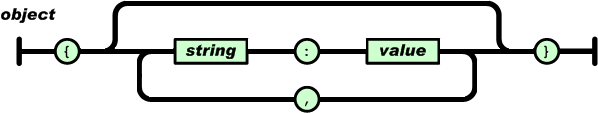
\includegraphics[scale=0.50]{icons/jsondoc.png}
      \caption{Oggetto JSON}
      \label{fig:jsondoc}
  \end{center}
\end{figure}
\\Un array è un insieme ordinato di valori. Un array comincia con una
parentesi quadra sinistra ``{[}'' e finisce con una parentesi destra``{]}''. I
valori sono separati da una~virgola~``,''~(Figura~\ref{fig:jsonarray}).
\begin{figure}[!h]
\begin{center}
    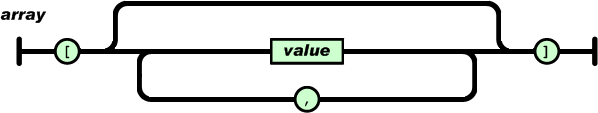
\includegraphics[scale=0.50]{icons/jsonarray.png}
    \caption{Array JSON}
    \label{fig:jsonarray}
\end{center}
Ogni nome di variabile è seguito dai due punti ``:'' e le coppie
``nome'' : ``valore'' sono separati
da una~virgola~``,''~(Figura~\ref{fig:jsonvalue}). In CouchDB assumono
significato particolare le variabili ``\_id'' e ``\_rev''. 

\end{figure}
\begin{figure}[!h]
  \begin{center}
      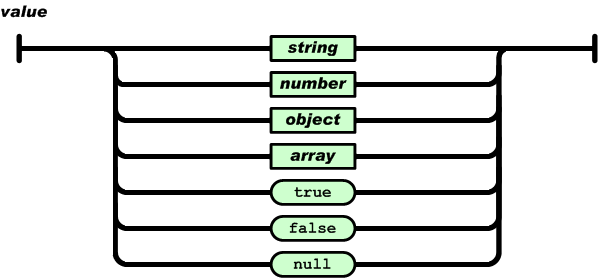
\includegraphics[scale=0.50]{icons/jsonvalue.png}
      \caption{Valore di una variabile JSON}
      \label{fig:jsonvalue}
  \end{center}
\end{figure}

\\L'oggeto utilizzato nel nostro modello è composto da sei variabili.
\emph{department} indica la facoltà per la quale è stata registrata una
votazione, il valore è una stringa univoca, nel caso la votazione si
riferisca ad un'operazione eseguita presso lo sportello veloce verrà registrata
con \emph{``sportello''}.\emph{Score} è una variabile numerica intera , nel
nostro modello può assumere i valori \{1,3,5\}.La data di effettuazione della
votazione,\emph{date} , viene raccolta dal sistema e salvata nel formato
``Y-m-d''.Gli attributi \emph{comment},\emph{customerName} e
\emph{customerEmail} nel caso il ciente lasci un feedback sono di tipo stringa , \emph{null} altrimenti. 
\\
\begin{lstlisting}[language=json] 
{ 
   _id:"182b00cd54a2b054fffabf1042000fbb", 
   _rev:"1-cb887f197900dce789c2dca898e4d330", 
   agency: "vicenza",
   operation: "counter",
   score: 5,
   date: "2013-06-01T11:40:52.280Z",
   comment: "Servizio efficiente",
   customerName: "Alex Tomasello",
   customerEmail: null
}
\end{lstlisting} 

\newpage
\subsection{API}
Il database è accessibile tramite richieste \acf{HTTP}, le cui proprietà sono
specificate nella \ac{RFC} 2616. Una richiesta
\ac{HTTP} è formata da una riga di richiesta (\emph{request line}) che contiene
il metodo, lo \ac{URI} e la versione del protocollo. La seconda componente della
richiesta è la sezione \emph{header} , la terza il \emph{body}. 

Attraverso i metodi messi a disposizione dal protollo,
è possibile memorizzare nuovi dati e creare nuove viste (\emph{Create}),
richiedere informazioni (\emph{Read}), modificare le informazioni memorizzate
all'interno dei documenti (\emph{Update}) ed eliminare documenti
(\emph{Delete}).

Ogni documento è raggiungibile da uno \ac{URL} univoco. Il protocollo \ac{HTTP}
prevede la seguente sintassi per definire l'~\ac{URL} di una risorsa alloccata : 

http\_URL = ``http:'' ``//'' host [ ``:'' port ] [ abs\_path [ ``?'' query
]]
\\
\emph{Host} è l'indirizzo del server sul quale è ospitato il database,
\emph{port} indica la porta sulla quale è in ascolto CouchDB, che di default è
la 5984 per richieste http, 6984 per ssl, modificabili accedendo al file di
configurazione. Se si vuole accedere al database \emph{abs\_path} è il nome del
database stesso, se si vuole accedere ad una vista il percorso da inserire sarà
composto da

nome\_database ``/\_design/'' nome\_design\_document ``/\_view/'' nome\_vista.
\\\\
Le operazioni \ac{CRUD}  sulle risorse sono
eseguibili tramite i seguenti metodi \ac{HTTP} ( gli esempi riportati sono stati
realizzati con il command line tool \textit{cURL}):
\begin{itemize}
  \item \textbf{GET} : richiede l'elemento specificato. Il formato dell'\ac{URL}
  definisce ciò che viene restituito: CouchDB può restituire elementi
  statici (ad esmepio viste), documenti di database e di configurazione.
  L'informazione viene restituita sotto forma di un documento \ac{JSON}.
  Per ottenere documenti non l'URL deve essere composto da :
  
  ``http://'' host ``:'' port ``/'' database ``/'' \_id
  
  es: \emph{curl -X GET ``http://atcustomersat:5984/padova/55090\ldots''}.
  
  Per ottenere elementi statici come le viste l'URL deve essere composto da:
  
  ``http://'' host ``:'' port  ``/'' database ``/\_design/''\_id 
  
  es: \emph{curl -X GET
  ``http://atcustomersat:5984/padova/\_design/consulting''}.
  
  \item \textbf{HEAD} : questo metodo viene utilizzato per ottenere
  l'intestazione \ac{HTTP} di una richiesta GET senza il corpo della risposta.
  Viene utilizzato per verificare l'esistenza di un oggetto senza richiederne il
  contenuto. In caso di documenti di grandi dimensioni, verificarne l'esistenza
  con il metodo HEAD velocizza notevolmente l'applicazione, in quanto non si
  deve aspettare che ritorni l'oggetto richiesto. L'\ac{URL} per accedere ai
  documenti ha la stessa sintassi di una richiesta GET.
   
  es: \emph{curl -X HEAD ``http://atcustomersat:5984/padova/55090\ldots''}
  \item \textbf{POST} : permette di inviare nuovi documenti al database di
  destinazione. In questo caso la richiesta POST deve avere come
  contenuto del body un documento \ac{JSON} valido.
  
  Per inviare un documento l'URL deve essere composto da:
  
  ``http://'' host ``:'' port ``/'' database 
  
  es : \emph{curl -X POST ``http://atcustomersat:5984/padova'' -H
  ``Content-Type:}
  \emph{application/json'' --data @scorecard.json}
  
  Dove \emph{scorecard.json} è un file contentente un documento json. 
  \item \textbf{PUT} : permette di inviare una risorsa specificata. In
  CouchDB il metodo PUT può essere utilizzato per creare nuovi dodumenti e
  database.
  
  es : \emph{curl -X PUT ``http://atcustomersat:5984/padova/123456798''}
  \emph{ -H ``Content-Type:application/json'' --data @scorecard.json}
  \item \textbf{DELETE} : cancella la risorsa specificata.
  
  es: \emph{curl -X DELETE ``http://atcustomersat:5984/padova/55090\ldots''}
\end{itemize}
Per aderire alle specifiche HTTP, è necessario, inoltre, che gli headers
siano settati e vengano forniti in modo da ottenere il formato e codifica
corretta. Gli headers essenziali sono \emph{Content~-~type} e \emph{Accept}.
\textbf{Content~-~type} specifica il tipo di contenuto dei dati che
vengono forniti nella richiesta. CouchDB accetta il formato JSON quindi l'header
sarà \emph{application/json}.
L'header \textbf{Accept}, invece, indica quali tipi di file sono accettati dal
client, in formato MIME (es: text/html). Solitamente sarà settato con
\emph{application/json}, \emph{*/*} se sono supportati tutti i tipi di file.
\\\\
Per realizzare interrogazioni parametrizzate, si usano le query-string. La
query-string è la parte di un URL che contiene dei dati da passare in input ad
un programma. Il carattere ``?'' apre la query-string, è utilizzato come
carattere speciale e non viene incluso nella query. Ogni argomento è formato da
una coppia chiave - valore. Alla chiave X si assegna il valore Y con il segno
``='' ed ogni argomento è separato da un altro con il carattere ``\&''. 
La sinstassi per realizzare una query string è, dunque, la seguente :

  
``?parametro1=valore1\&parametro2=valore2\&parametro3=valore3''.
\\\\
Le query parametrizzate vengono utilizzate nell'applicazione nel momento della
generazione dei grafici. C'è la possibilità di scegliere la sede che si vuole
monitorare, il tipo di servizio, l'intervallo temporale e il tipo di grafico.
Ogni voce scelta andrà a settare un parametro nell'\ac{URL}. I parametri
permessi da CouchDB sono illustrati nella tabella seguente.
\\\\
\begin{tabular}{|>{\columncolor{background}}p{2.4cm}|p{3.1cm}|p{1.4cm}|p{5.8cm}|}
  \hline
  \rowcolor{table}
  \textbf{Parametro} & 
  \textbf{Valore} & 
  \textbf{Default} &
  \textbf{Descrizione}
   
  \\\hline key & JSON & - & Indica la coppia chiave-valore, deve rispettare
  la sintassi dell'URL.
  \\\hline startkey & JSON
    & - & Indica il valore della chiave di partenza, deve rispettare la
    sintassi dell'URL.
  \\\hline startkey\_docid & ``\_id'' del documento & - & ID del documento di
  partenza.
  \\\hline endkey & JSON
    & - & Indica il valore massimo della chiave, deve rispettare la
    sintassi dell'URL.
  \\\hline endkey\_docid & ``\_id'' del documento & - & ID del documento che
    termina la ricerca.
  \\\hline limit & intero & - & Limita il numero di documenti
    restituiri.
  \\\hline descending & true/false & false & Ordinamento della ricerca.
  \\\hline skip & intero & 0 & Salta il numero indicato di documenti.
  \\\hline group & true/false & false & Controlla se la funzione di
    \emph{reduce} viene applicata a un gruppo di chiavi distinte o singola riga di
    risultati.
  \\\hline group\_level & intero & - & Indica il livello di raggruppamento da
  applicare alla funzione \emph{reduce}.
  \\\hline reduce & trey/false & true & Specifica se utilizzare la funzione
  \emph{reduce}.
  \\\hline
\end{tabular}
\\\\
Ad esempio per ricevere i dati di una particolare sede, ragguppati per mesi e
per il periodo temporale compreso tra gennaio e luglio 2013, la query è la
seguente

?group\_level=2\&startkey=[2013,1,1,1]\&endkey=[2013,7,31,23]
\newpage
\subsection{Replication} 
CouchDB consente si sincronizzare database situati su differenti host
permettendo quindi agli utenti di accedere a risorse situate su host diversi in
modo trasparente.
La sincronizzazione è possibile perchè CouchDB è un database
NOSQL e quindi ogni base di dati è una collezione di documenti indipendenti tra
di loro, cioè che documenti diversi possono rappresentare oggetti
diversi.
La sincronizzazione è unilaterale, bisogna indicare un server che conterrà
il database originale (\emph{source}) e uno con funzione di \emph{target}.
Un database viene definito ``locale'' quando si trova sulla stessa istanza del
server al quale viene inviata la richiesta di replication.
Tutti gli altri casi i database sono definiti ``remoti''.
Per sincronizzare un database si effettua una richiesta POST, inviando nel body
un documento JSON contenente i database di source e destination:

\begin{lstlisting}[language=json]
//file replication.json:
{
  source:"database",
  target:"http://example.org/database"
}
\end{lstlisting}
 
 
\emph{curl -X POST http://atcustomersat:5984/\_replicate -H ``Content-Type:}
\emph{application/json'' --data @replication.json}
\\\\
Quando si utilizza la sincronizzazione, CouchDB confronta i due database e
verifica quali documenti presenti nel source differiscono da quelli presenti nel
target. I documenti alloccati nel target verranno modificati , cancellati o
creati a seconda dello stato di quelli presenti nell'origine. Il numero di
revisione del documento viene modificato, ed è possibile risalire alle modifiche
effettuate al momento della sincronizzazione. Per realizzare una
sincronizzazione bilaterale basta inviare due richieste di replication
invertendo target e source.

Aggiungendo il parametro continuous e settandolo a true, è possibile continuare
a sincronizzare i database ogni volta che vengono aggiunti o modificati
documenti nel database di source. Nell'attuale versione di CouchDB ( v1.3.0) non
è possibile continuare la sincronizzazione dopo il riavvio del server, in quanto
i settaggi della replication vengono resettati.

\newpage
\subsection{Map-Reduce}
\emph{MapReduce} è un framework software per scrivere facilmente applicazioni
che elaborano grandi quantità di dati in parallelo. Il sistema è formato da due
funzioni~: \emph{map} e \emph{reduce}. La prima elabora le coppie chiave-valore
, la seconda elabora il set di coppie generate dalla funzione \emph{map} 
restituendo l'output richiesto.
\begin{itemize}
  \item \emph{map}: il nodo master prende i dati di ingresso (fase
  \emph{input}), li suddivide in piccoli blocchifase
  \emph{splitting}, generalmente da 64MB o 128MB e distribuisce il lavoro ai
  nodi slaves. Il singolo nodo \emph{mapper} produce il risultato intermedio della
  funzione di map() sotto forma di coppie [chiave,valore] memorizzate su un file
  distribuito, la cui locazione è notificata al master alla fine della fase di
  map (fase \emph{mapping}).
  \item \emph{reduce}: il nodo master colleziona le risposte, combina le coppie
  [chiave,valore] in liste di valori che condividono la stessa chiave e li
  ordina per chiave (fase
  \emph{shuffling}). Le coppie della forma,
  [chiave,IteratorList(valore,\ldots)] sono passate ai nodi reducer che
  eseguono la funzione di reduce() (fase
  \emph{reducing}).
\end{itemize}
Le funzioni di \emph{map} e \emph{reduce} sono implementate in Javascript, e
CouchDB mette a disposizione ulteriori funzioni native da utilizzare.
La funzione \emph{reduce} come parametri di input ha una collection di chiavi,
una collection di valori e un valore booleano \emph{rereduce}. Se settato a
true, rereduce permette di usare la funzione reduce al blocco di risultati
generato dalle chiamate della funzione. Per database di grandi dimensioni,
CouchDB chiama le funzioni per blocchi di dati in modo da velocizzare l'analisi
dei dati. Non applicando la funzione rereduce c'è il rischio di ottenere un
output sbagliato.

 Ad esempio ipotizziamo di avere un set di documenti
composto da 1000 chiavi.
La fase di map calcola ``chiave''=``valore'' e il motore di CouchDB divide i
documenti ricevuti come input in 3 blocchi. Nella fase di reduce, la funzione
calcola quanti elementi sono presenti nel db. La situazione di partenza prevede
1000 oggetti, la fase di map e reduce divide in 3 blocchi contenenti
rispettivamente 333,333 e 334 oggetti.
L'output resituito dalla funzione reduce è errato, in quanto calcola il numero
di oggetti presenti restituito dopo le operazioni, calcola quindi 3
oggetti(~Figura~\ref{fig:reduce}).
Applicando la funzione di rereduce, invece, viene calcolata la somma dei valori
restituiti dai 3 oggetti temporanei, restituendo l'output
corretto(~Figura~\ref{fig:rereduce}).


\begin{figure}[!h]
\begin{tikzpicture}[%
  >=triangle 60,              % Nice arrows; your taste may be different
  start chain=going below,    % General flow is top-to-bottom
  node distance=6mm and 60mm, % Global setup of box spacing
  every join/.style={norm},   % Default linetype for connecting boxes
  ]
\tikzset{
  base/.style={draw, on chain, on grid, align=center, minimum height=4ex},
  proc/.style={base, rectangle, text width=10em},
  map/.style={base, rectangle, text width=10em},
  cong/.style={->, draw, lccong}, 
  it/.style={font={\small\itshape}}
}
\node
[proc,xshift=12em](input){\textbf{key}~,~\textbf{val}\\1~,~1\\\ldots~,\ldots\\1000~,~5984};
\node [proc,xshift=-12em](split1){\textbf{key}~,~\textbf{val}\\1~,~1\\\ldots~,
\ldots\\333,210};
\node [map,fill=background](map1){function(key,val)~\{\\ count(val);\}};
\node [proc](result1){\textbf{key} , \textbf{val}\\ null~,~333};
\node [proc,xshift=12em,yshift=15.19em](split2){\textbf{key}
,\textbf{val}\\334~, 458\\\ldots~,~\ldots\\666,131}; 
\node [map,fill=background](map2){function(key,val)~\{\\ count(val);\}}; 
\node [proc](result2){\textbf{key} , \textbf{val}\\ null~,~333}; 
\node [proc,xshift=12em,yshift=15.19em](split3){\textbf{key}
,\textbf{val}\\667~,~125\\\ldots~,\ldots\\1000,5984}; 
\node [map,fill=background](map3){function(key,val)~\{\\ count(val);\}}; 
\node [proc](result3){\textbf{key} ,\textbf{val}\\ null~,~334};
\node [map,fill=background,xshift=-12em](reduce){function(key,val)~\{\\ count(val);\}};
\node [proc](output){\textbf{key} , \textbf{val}\\null~,~3};

\path (input.south) to node [near start, xshift=5em] {}
(split1); \draw [->] (input.south) -- (split1.north);
\path (input.south) to node [near start, xshift=5em] {}
(split2); \draw [->] (input.south) -- (split2.north);
\path (input.south) to node [near start, xshift=5em] {}
(split3); \draw [->] (input.south) -- (split3.north);

\path (split1.south) to node [near start, xshift=5em] {}
(map1); \draw [->] (split1.south) -- (map1.north);
\path (split2.south) to node [near start, xshift=5em] {}
(map2); \draw [->] (split2.south) -- (map2.north);
\path (split3.south) to node [near start, xshift=5em] {}
(map3); \draw [->] (split3.south) -- (map3.north);

\path (map1.south) to node [near start, xshift=5em] {}
(result1); \draw [->] (map1.south) -- (result1.north);
\path (map2.south) to node [near start, xshift=5em] {}
(result2); \draw [->] (map2.south) -- (result2.north);
\path (map3.south) to node [near start, xshift=5em] {}
(result3); \draw [->] (map3.south) -- (result3.north);

\path (result1.south) to node [near start, xshift=5em] {}
(reduce); \draw [->] (result1.south) -- (reduce.north);
\path (result2.south) to node [near start, xshift=5em] {}
(reduce); \draw [->] (result2.south) -- (reduce.north);
\path (result3.south) to node [near start, xshift=5em] {}
(reduce); \draw [->] (result3.south) -- (reduce.north);

\path (reduce.south) to node [near start, xshift=5em] {}
(output); \draw [->] (reduce.south) -- (output.north);

\end{tikzpicture} 
\caption{MapReduce con \emph{rereduce=false}}\label{fig:reduce}
\end{figure}

\def\HS{\hspace{\fontdimen2\font}}

\begin{figure}[!h]
\begin{tikzpicture}[%
    >=triangle 60,              % Nice arrows; your taste may be different
    start chain=going below,    % General flow is top-to-bottom
    node distance=6mm and 60mm, % Global setup of box spacing
    every join/.style={norm},   % Default linetype for connecting boxes
    ]
\tikzset{
  base/.style={draw, on chain, on grid, align=center, minimum height=4ex},
  empty/.style={ on chain, on grid, align=center, minimum height=6ex,text
  width=10em},
  proc/.style={base, rectangle, text width=10em, align=center},
  map/.style={base, rectangle, text width=10em,align=left},
  cong/.style={->, draw, lccong}, 
  it/.style={font={\small\itshape}}
}
\node [empty, densely dotted, it] (empty1) { };
\node [proc, densely dotted, it,xshift=12em] (p0) { splitting \space  \&
\space mapping }; \node [map,fill=background](reduce){function(key,val)~\{\\
if (rereduce)\\ \{\space\space\space sum(val) \} \\ else\\
\{\space\space\space count(val) \};\}}; \node [proc](output){\textbf{key} ,
\textbf{val}\\null~,~1000};

\path (p0.south) to node [near start, xshift=5em] {}
(reduce); \draw [->] (p0.south) -- (reduce.north);

\path (reduce.south) to node [near start, xshift=5em] {}
(output); \draw [->] (reduce.south) -- (output.north);

\end{tikzpicture} 
\caption{MapReduce con \emph{rereduce=true}}\label{fig:rereduce}
\end{figure}



\newpage \newpage
Di seguito è presentata la funzione map utilizzata nel calcolo della somma dei
voti per l'operazione di consulenza. Nel momento della fase di map, vengono scartati
i documenti che non appartengono al gruppo scelto. Successivamente viene creata
la coppia chiave-valore da inviare alla funzione di reduce. La chiave è la data
trasformata in un array, per agevolare il raggruppamento in fase di output.

\begin{lstlisting}[language=JavaScript] 
function(doc) {
  if (doc.operation != 'consulting') 
    return;
  var date = new Date(doc.date);
  emit(
    [date.getFullYear(), 
     (date.getMonth()  +1),
     date.getDate(),
     date.getHours()],
    doc.score); 
}
\end{lstlisting}
La funzione reduce raccoglie i dati, distinguendo i casi in cui rereduce è
settato a true oppure a false.
 \begin{lstlisting}[language=JavaScript]
function (key, values, rereduce) {
  // Reduce function
  var count = 0;
  var sum = 0;
  var i;

  if(!rereduce) {
    // `values` stores actual map output
    for(i = 0; i < values.length; i++) {
      count += 1;
      sum += Number(values[i]);
    }
    return {"count":count, "sum":sum};
  }

  else {
    // `values` stores count/sum objects returned previously.
    for(i = 0; i < values.length; i++) {
      count += values[i].count;
      sum   += values[i].sum;
    }
    return {"count":count, "sum":sum};
  }
}
\end{lstlisting}


\newpage
\section{Promise Pattern}
Per registrare il voto espresso dall'utente si effettua una richiesta POST al
server dove è ospitato il dabatase. Le richieste vengono inoltrate con
metodologia \ac{AJAX}. \ac{AJAX} permette di
effettuare delle chiamate asincrone, cioè chiamate ad una risorsa
esterna che non interferiscono con l'esecuzione della risorsa chiamante. I
risultati della risorsa esterna saranno utilizzabili solo quando disponibili.
Chiamate di tipo asincrono, quindi, permettono di effettuare altre operazioni
senza alcun redirect o refresh della pagina.

La richiesta HTTP viene composta dal metodo \$.ajax() prendendo in
considerazione i parametri d'ingresso. Settando il metodo da chiamare, gli
header necessari e il body, la richiesta viene composta e inviata al server.
Utilizzare chiamate asicnrone, permette di strutturare il codice in nuovo modo:
mentre le richieste \ac{AJAX} vengono eseguite è possibile realizzare delle
callback che possono essere chiamate a seconda dello stato della chiamata
utilizzando il promise pattern. 

Una promessa è un oggetto che rappresenta il valore di ritorno o l'eccezione
lanciata che una funzione può eventualmente fornire. Il promise pattern prevede
tre differenti stati di una promessa :
soddisfatta ( \emph{fulfilled} ) nel caso in cui la funzione ritorni un valore,
non soddisfatta ( \emph{rejected} ) nel caso la funzioni generi un'eccezione e in
corso ( \emph{progress}).
Lo stato progess è uno stato temporaneo, mentre fulfilled e rejected sono
definitivi. Una promessa può passare da uno stato progess a uno degli
altri due, ma non viceversa. Il costrutto delle promesse permette quindi di
realizare delle funzioni che vengono chiamate a seconda dello stato
dell'oggetto. Le funzioni sono create all'interno del metodo
then(~doneCallbacks [, failCallbacks] [, progressCallbacks ]~) riferito alla
funzione iniziale.

Con l'uso delle promesse la scrittura del codice viene semplificata ed agevola
il controllo degli errori. Se pensiamo ad una serie di eventi da realizzare in
catena, una funzione viene scritta all'interno dell'altra, e richiede
particolare attenzione dal parte del programmatore per evitare gli errori. Ad
esempio il codice:
\\\\
\begin{lstlisting}[language=JavaScript] 
step1(function (value1) {
    step2(value1, function(value2) {
        step3(value2, function(value3) {
            step4(value3, function(value4) {
                // Do something with value4
            });
        });
    });
}); 
\end{lstlisting}
può essere semplificato con le promesse. Lo stato di una promessa viene
propagato, quindi possiamo cogliere il fallimento di una di esse nel
momento in cui fallisce, o alla fine della catena di promesse. In
questo caso possiamo riscrivere il codice presentato prima con il seguente:
\\\\
\begin{lstlisting}[language=JavaScript] Q.fcall(step1) .then(step2)
.then(step3)
.then(step4)
.then(function (value4) {
    // Do something with value4
}, function (error) {
    // Handle any error from step1 through step4
})
.done();
\end{lstlisting}
L'utilizzo delle promesse facilita anche l'utilizzo di chiamate parallele. Il
metodo \emph{all} riceve un array di promesse, ed appena tutte
sono risolte si scatenano gli eventi della callback. In altri casi è possibile
attendere che solo una di un array di promesse venga soddisfatta e si utilizza
allora il metodo \emph{any}. Un'ulteriore alternativa consiste nell'attendere un
numero precisato di promesse soddisfatte utilizzando la funzione \emph{some}.
\\\\
Di seguito il codice utilizzato nell'applicazione per inviare la votazione.
Il metodo ajax() riceve come parametri d'ingresso l'URL del server,   
il metodo \ac{HTTP} e l'oggetto da memorizzare nella base di dati. In questo
caso la promessa, quando e se viene soddisfatta, lancia la funzione che restituisce un
feddback all'utente della corretta esecuzione del processo di voto. 

 \begin{lstlisting}[language=JavaScript] 
$.ajax('http://' + server +':8888/' + agency, { 
    type : "POST",
    contentType : "application/json",
    processData : false,
    data : JSON.stringify({
      "agency" : agency,
      "operation" : operation,
      "score" : $(this).data('score'),
      "date" : new Date(),
      "comment" : $('#comment').val(),
      "customerName" : $('#customerName').val(),
      "email" : $('#email').val()
    })
  }).then(function(response) {
      $('#feedback').modal({
        backdrop : 'static'
      });
    });
\end{lstlisting}

\clearpage{\pagestyle{plain}\cleardoublepage}
\chapter{Conclusioni}
\label{cha:conclusioni}
Le modalità di sviluppo e la scelta degli strumenti, hanno premesso di creare
un'applicazione modulare. Modelli e procedure sono state più volte modificate
nel corso della progettazione e implementazione. La scelta di usare un database
non relazionale, di aderire al pattern architetturale \acf{MVC} e al promise
pattern ha permesso di elaborare un'applicazione solida e facilmente
modificabile. 

Il modello stesso dei dati salvato nel database
CouchDB è stato più volte cambiato, aggiungendo e modificando proprietà
dell'oggetto senza riscontrare difficoltà nella definizione dei tipi di dati.
Diversamente sarebbe stato se avessi utilizzato un database relazionale. CouchDB
si è dimostrato una scelta valida anche per quanto riguarda la sincronizzazione
dei dati. Trovandosi di fronte a una situzione in cui più host dovevano
dialogare fra di loro, i metodi, facilmente configurabili, messi a disposizione
dal database hanno agevolato il passaggio di dati fra sede centrale e filiali.

La struttura aderente al pattern \ac{MVC} a promise pattern, invece, permette di
inserire nuove azioni che vanno a dialogare con i modelli. Ogni funzione viene
implementata in modo indipendente dalle altre, in quanto lo stato di una
promessa può essere fulfilled, restituendo il contenuto, oppure rejected.
Funzioni concatenate fra loro devono solo gestire i due casi appena citati.
Saranno implementate nuove funzioni per gestire il login per gli amministratori
al momento della visualizzazione dei grafici.
Questa sezione verrà implementata utilizzando un proprio framework \ac{PHP} in
fase di sviluppo che gestirà la fase di autenticazione, implementazione di \ac{ACL} e
la sicurezza dei dati. Ulteriori funzionalità verranno aggiunta per quando
riguarda l'analisi dei dati, permettendo di confrontare fra loro più sedi.
L'utilizzo di richieste \acf{AJAX} parallele consente già di
ottenere tutti i dati necessari per la composizione di nuovi grafici.

L'applicazione ha soddisfatto le attese del cliente committente e allo stato
attuale è installata in versione di prova in alcune sedi. Si è cercato inoltre
di implementare il codice in modo da lasciare ampio spazio alle customizzazioni,
così da ottenere un modello valido anche per altre utilizzazioni future. 
\newpage
\section{screenshot}
  \begin{figure}[!h]
    \begin{center}
      
\includegraphics[scale=0.30]{icons/screen_intro.png}
      \caption{Schermata introduttiva}
      \label{fig:screen_intro}
    \end{center}
  \end{figure}
  \begin{figure}[!h]
    \begin{center}
      
\includegraphics[scale=0.30]{icons/screen_voting.png}
      \caption{Scelta del livello di soddisfazione}
      \label{fig:screen_voting}
    \end{center}
  \end{figure}
  \begin{figure}[!h]
    \begin{center}
      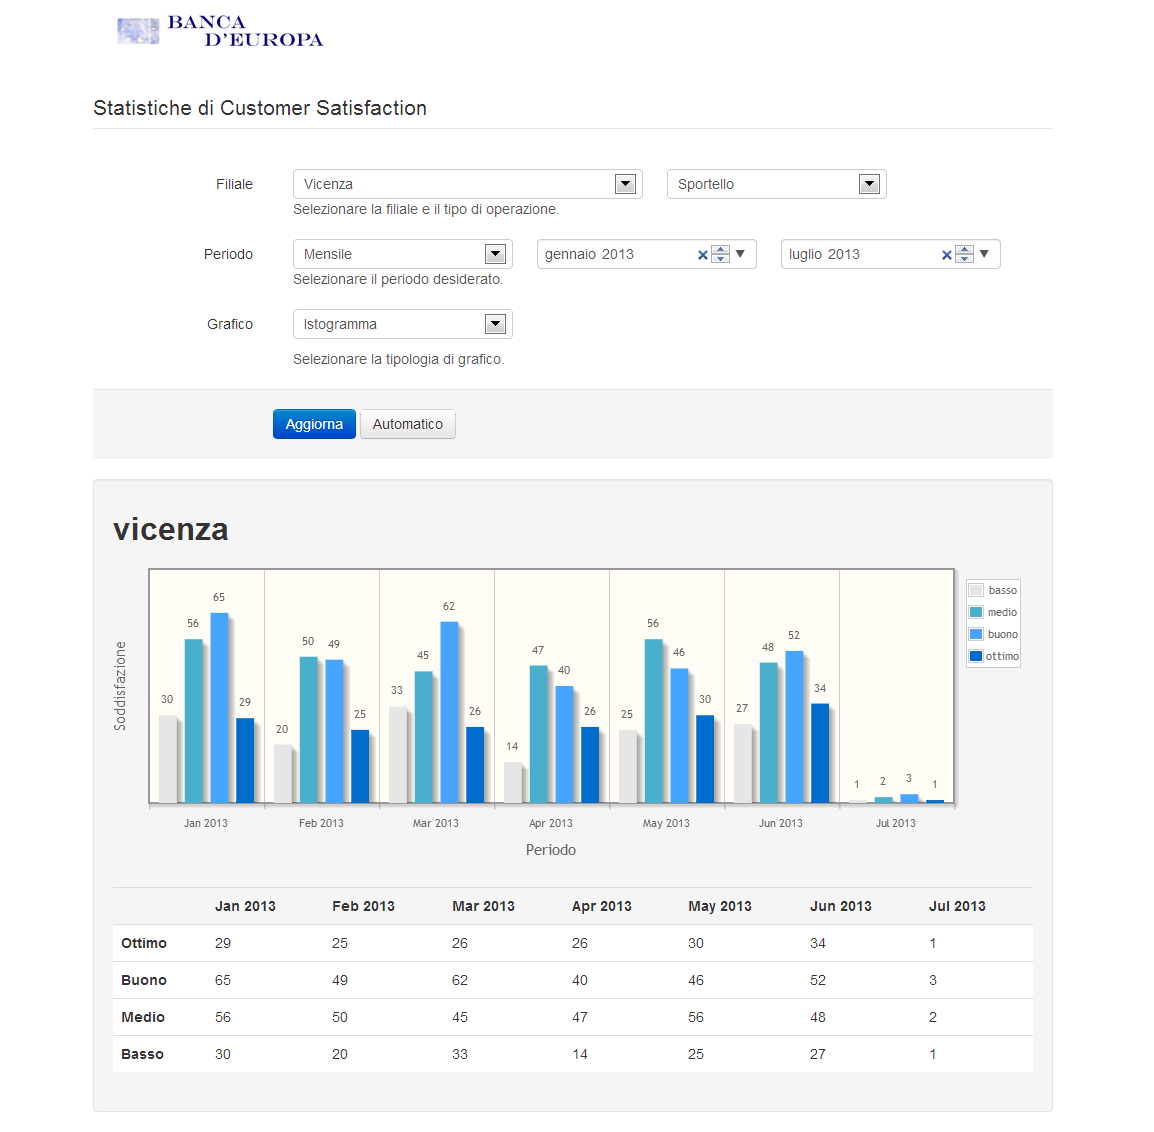
\includegraphics[scale=0.35]{icons/screen_graph.png}
      \caption{Generazione dei grafici}
      \label{fig:screen_graph}
    \end{center}
  \end{figure}

\clearpage{\pagestyle{plain}\cleardoublepage}
\chapter{Bibliografia e sitografia}
\label{cha:bibliografia}
\begin{itemize}
  \item Zeithaml Parasuraman Berry, \emph{Delivering Quality Service: Balancing
  Customer Perceptions and Expectations}, Free Press, 2009
  \item Busacca B., \emph{Le risorse di fiducia dell’impresa: soddisfazione del
  cliente, creazione del valore strategie di accrescimento}, Utet, 1994
  \item http://wiki.apache.org/couchdb/Reference
  \item http://couchdb.readthedocs.org/en/latest/
  \item https://github.com/kriskowal/q/
  \item http://www.ensta-paristech.fr/~kielbasi/tikzuml/index.php?lang=en
  \item http://en.wikipedia.org/wiki/Unified\_Modeling\_Language
  \item http://research.google.com/archive/mapreduce.html
  \item http://api.jquery.com/jQuery.ajax/
  \item http://tools.ietf.org/html/rfc2616
  \item http://www.json.org/
  \item http://en.wikipedia.org/wiki/Model-View-Controller
\end{itemize}

\clearpage{\pagestyle{plain}\cleardoublepage}
\chapter{Acronimi}
\label{cha:acronimi}
\acrodef{CS}[CS]{Customer Satisfaction}
\acrodef{HTML}[HTML]{HyperText Markup Language}
\acrodef{CSS}[CSS]{Cascading Style Sheets}
\acrodef{JS}[JS]{JavaScript}
\acrodef{DBMS}[DBMS]{Database Management System}
\acrodef{HTTP}[HTTP]{HyperText Transfer Protocol}
\acrodef{MVC}[MVC]{Model View Controller}
\acrodef{CouchDB}[CouchDB]{Cluster Of Unreliable Commodity Hardware}
\acrodef{NoSQL}[NoSQL]{Not Only SQL}
\acrodef{JSON}[JSON]{JavaScript Object Notation}
\acrodef{MCC}[MCC]{Multiversion Concurrency Control}
\acrodef{ACID}[ACID]{Atomicity Consistency Isolation Durability}
\acrodef{API}[API]{Application Programming Interface}
\acrodef{RFC}[RFC]{Request for Comments}
\acrodef{URI}[URI]{Uniform Resource Identifier}
\acrodef{URL}[URL]{Uniform Resource Locator}
\acrodef{CRUD}[CRUD]{Create Read Update Delete}
\acrodef{AJAX}[AJAX]{Asynchronous JavaScript and XML}
\acrodef{ACL}[ACL]{Access Control List}
\acrodef{PHP}[PHP]{PHP: Hypertext Preprocessor}


\acf{CS}\\
\acf{HTML}\\
\acf{CSS}\\
\acf{JS}\\
\acf{DBMS}\\
\acf{HTTP}\\
\acf{MVC}\\
\acf{CouchDB}\\
\acf{NoSQL}\\
\acf{JSON}\\
\acf{MCC}\\
\acf{ACID}\\
\acf{API}\\
\acf{RFC}\\
\acf{URI}\\
\acf{URL}\\
\acf{CRUD}\\
\acf{AJAX}\\
\acf{ACL}\\
\acf{PHP}\\

\end{document}
